\begin{figure}
  \def\frac{0.24}
  \rotatebox{90}{{\tiny \hspace{0.5cm} \color{blue}{Hand Reach}}}%
  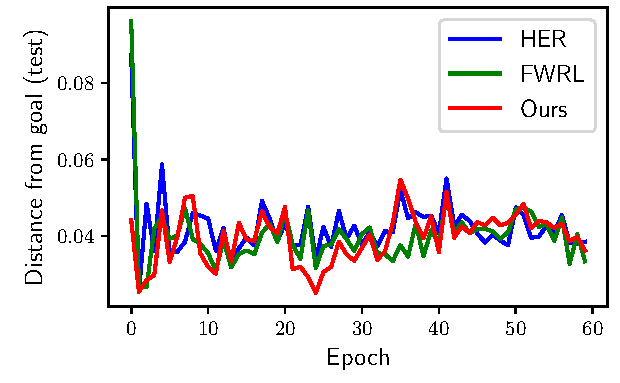
\includegraphics[width=\frac\columnwidth]{media/res/6efc1de-path_reward_low_thresh_chosen-HandReachPR-v0-dqst/epoch-test/ag_g_dist.pdf}%
  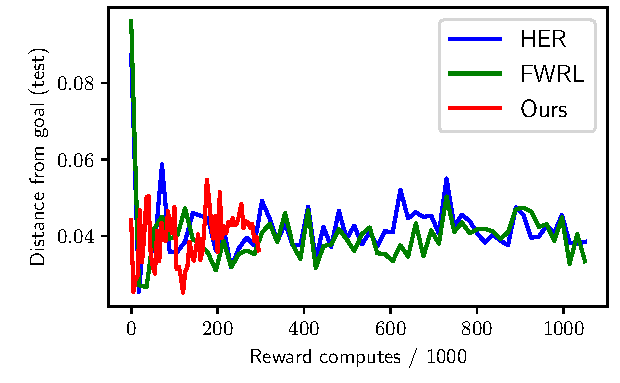
\includegraphics[width=\frac\columnwidth]{media/res/6efc1de-path_reward_low_thresh_chosen-HandReachPR-v0-dqst/reward_computes-test/ag_g_dist.pdf}%
  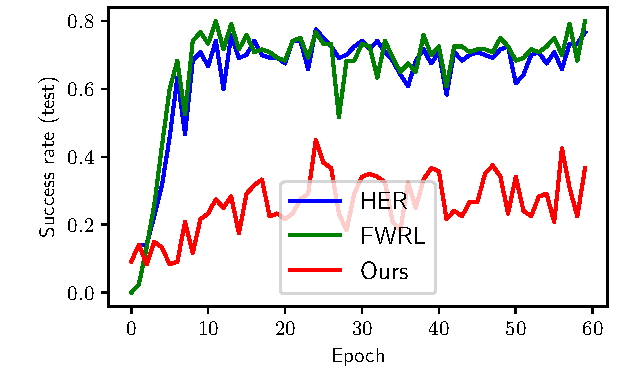
\includegraphics[width=\frac\columnwidth]{media/res/6efc1de-path_reward_low_thresh_chosen-HandReachPR-v0-dqst/epoch-test/success_rate.pdf}%
  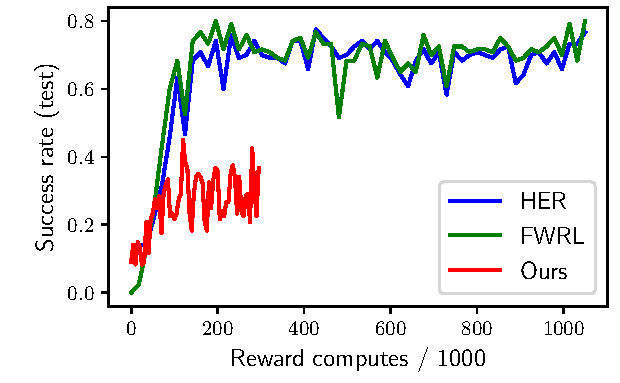
\includegraphics[width=\frac\columnwidth]{media/res/6efc1de-path_reward_low_thresh_chosen-HandReachPR-v0-dqst/reward_computes-test/success_rate.pdf}\\
  \rotatebox{90}{{\tiny \hspace{1em} \color{blue}{Hand Block Rotate}}}%
  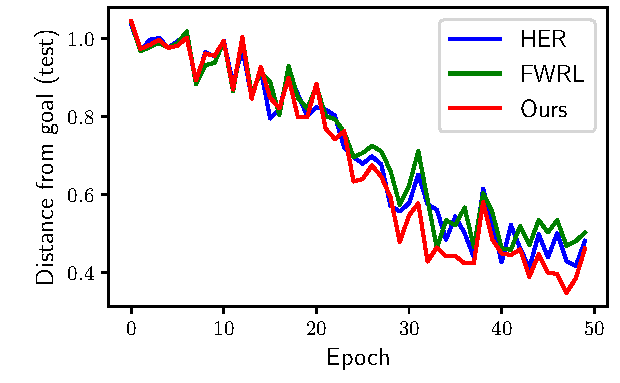
\includegraphics[width=\frac\columnwidth]{media/res/6efc1de-path_reward_low_thresh_chosen-HandManipulateBlockRotateXYZPR-v0-dqst/epoch-test/ag_g_dist.pdf}%
  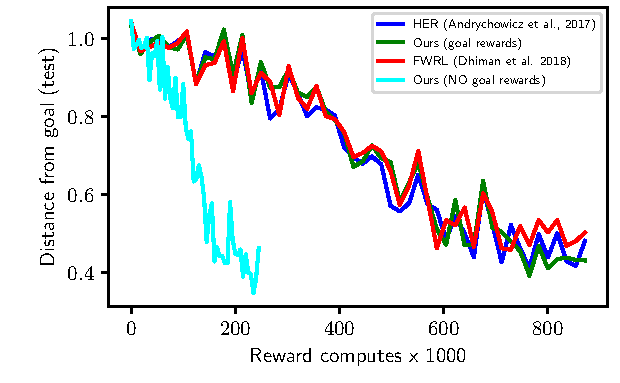
\includegraphics[width=\frac\columnwidth]{media/res/6efc1de-path_reward_low_thresh_chosen-HandManipulateBlockRotateXYZPR-v0-dqst/reward_computes-test/ag_g_dist.pdf}%
  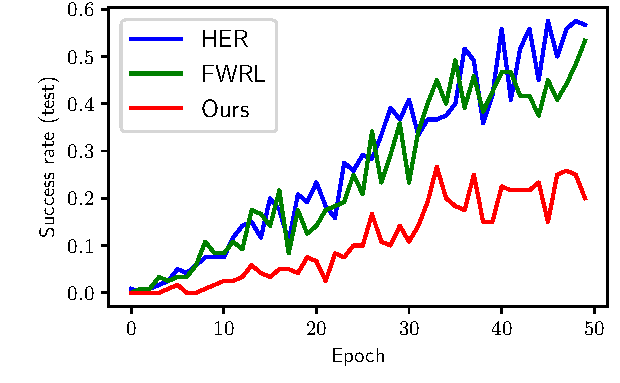
\includegraphics[width=\frac\columnwidth]{media/res/6efc1de-path_reward_low_thresh_chosen-HandManipulateBlockRotateXYZPR-v0-dqst/epoch-test/success_rate.pdf}%
  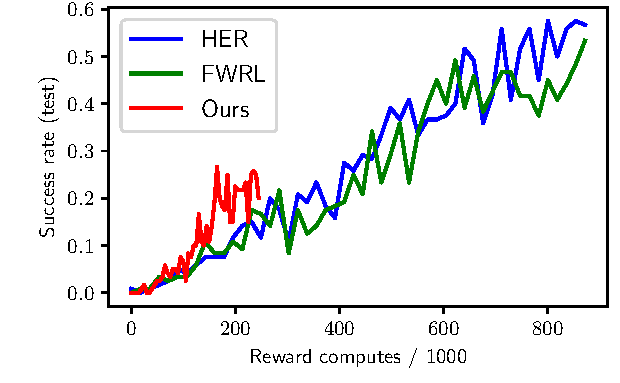
\includegraphics[width=\frac\columnwidth]{media/res/6efc1de-path_reward_low_thresh_chosen-HandManipulateBlockRotateXYZPR-v0-dqst/reward_computes-test/success_rate.pdf}\\
  \rotatebox{90}{{\tiny \hspace{0.7cm} \color{blue}{Hand Egg}}}%
  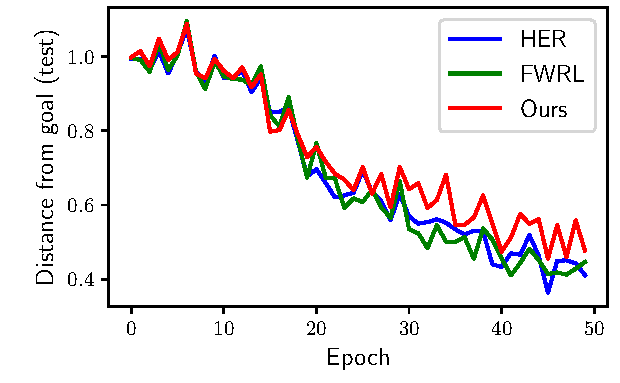
\includegraphics[width=\frac\columnwidth]{media/res/6efc1de-path_reward_low_thresh_chosen-HandManipulateEggFullPR-v0-dqst/epoch-test/ag_g_dist.pdf}%
  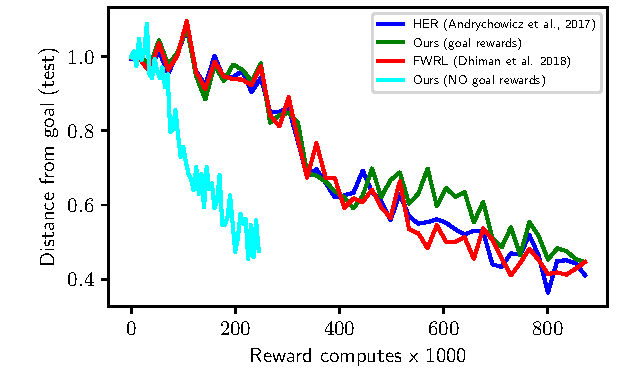
\includegraphics[width=\frac\columnwidth]{media/res/6efc1de-path_reward_low_thresh_chosen-HandManipulateEggFullPR-v0-dqst/reward_computes-test/ag_g_dist.pdf}%
  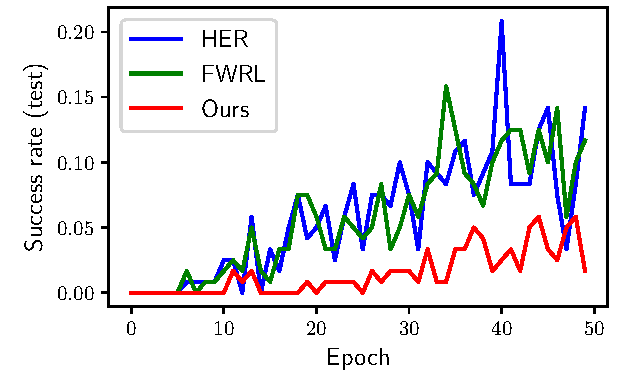
\includegraphics[width=\frac\columnwidth]{media/res/6efc1de-path_reward_low_thresh_chosen-HandManipulateEggFullPR-v0-dqst/epoch-test/success_rate.pdf}%
  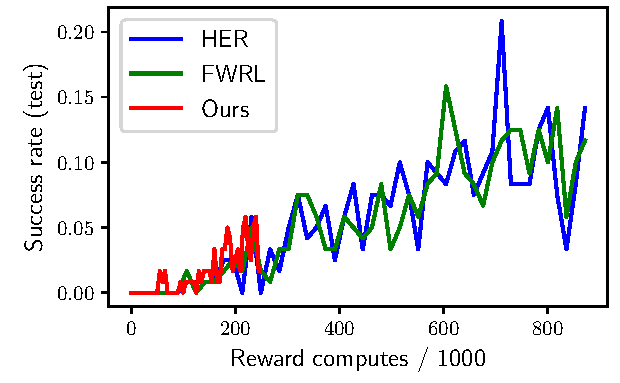
\includegraphics[width=\frac\columnwidth]{media/res/6efc1de-path_reward_low_thresh_chosen-HandManipulateEggFullPR-v0-dqst/reward_computes-test/success_rate.pdf}\\
  \rotatebox{90}{{\tiny \hspace{0.5cm} \color{blue}{Hand Pen Rotate}}}%
  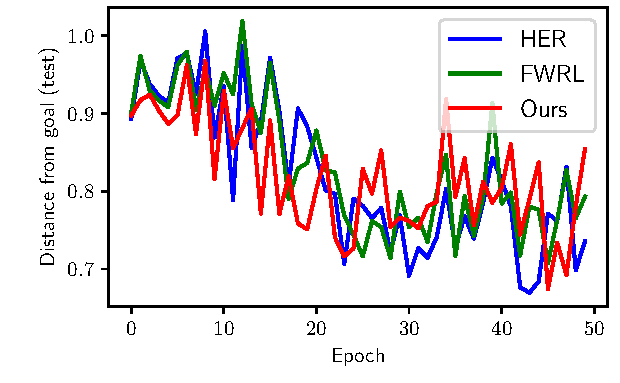
\includegraphics[width=\frac\columnwidth]{media/res/6efc1de-path_reward_low_thresh_chosen-HandManipulatePenRotate-v0-ddpg/epoch-test/ag_g_dist.pdf}%
  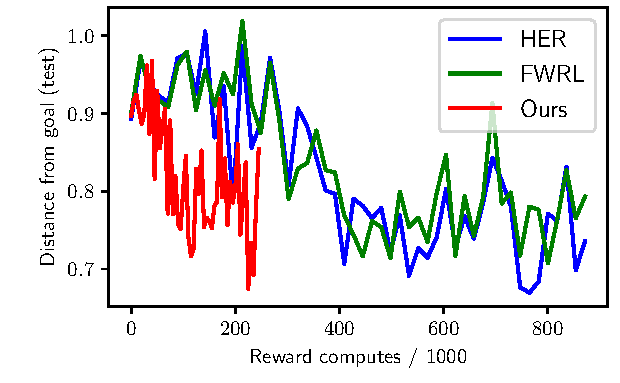
\includegraphics[width=\frac\columnwidth]{media/res/6efc1de-path_reward_low_thresh_chosen-HandManipulatePenRotate-v0-ddpg/reward_computes-test/ag_g_dist.pdf}%
  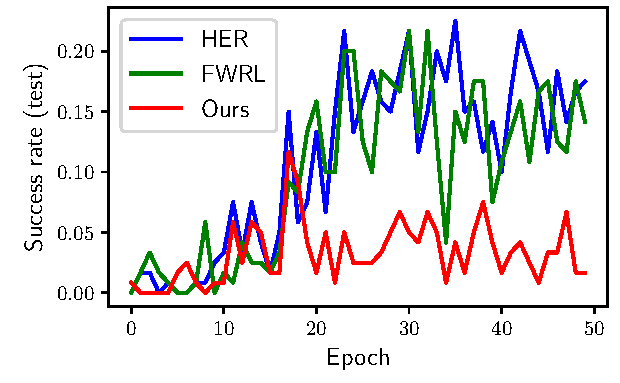
\includegraphics[width=\frac\columnwidth]{media/res/6efc1de-path_reward_low_thresh_chosen-HandManipulatePenRotate-v0-ddpg/epoch-test/success_rate.pdf}%
  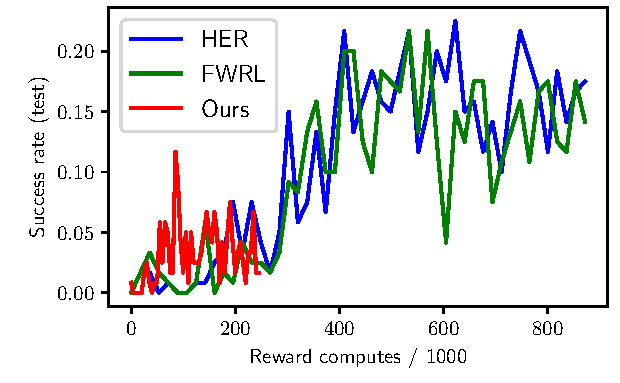
\includegraphics[width=\frac\columnwidth]{media/res/6efc1de-path_reward_low_thresh_chosen-HandManipulatePenRotate-v0-ddpg/reward_computes-test/success_rate.pdf}
  {.\tiny\color{blue}\hspace{0.8cm}(a) Distance on Epochs \hspace{1.05cm}(b) Distance on
    reward computes
    \hspace{0.70cm} (c) Success rate on epochs \hspace{0.9cm} (d) Success rate on reward computes}
  \caption{For the hand tasks, we compare our method (red) against HER (blue) ~\citep{andrychowicz2016learning}
    and FWRL (green) ~\citep{dhiman2018floydwarshall} for the distance-from-goal
    and success rate metrics. Furthermore, both metrics are plotted
    against two progress measures, the number of training epochs and the number of reward
    computations. Measured by distance from the goal, our method performs comparable to or
    better than the baselines for both progress measurements. For the success rate,
    our method underperforms against the baselines. 
}%
  \label{fig:hand-results}%
\end{figure}%
% 
